\section{Overview}
	
	Section \ref{revisedspec} introduced the overall abstract components of the system. The design is based on this 
	principle to provide an extensible gaming platform, fully implementing the requirements for the particular
	behavior of \emph{6.170 Antichess} with ease. 
	
	In order to fully appreciate the extensibility provided by \emph{Pawned}, it is useful to consider the execution environment 		as separated from the implementation of  \emph{6.170 Antichess}. With this environment, it is possible to describe a broad 		
	range of sequential games using the execution environment as a platform. 

\section{Game Execution Environment}
	
	The game execution environment publishes a set of interfaces that enables a Java programmer to fully implement a sequential 
	board game by indicating the rules and pieces for their game. Based on the functionality of these implemented interfaces,
	the \emph{Game Execution Environment} is then capable to execute a game successfully. The structure of this platform can 
	be divided into four independent layers. 

		\begin{figure}
			\begin{center}
				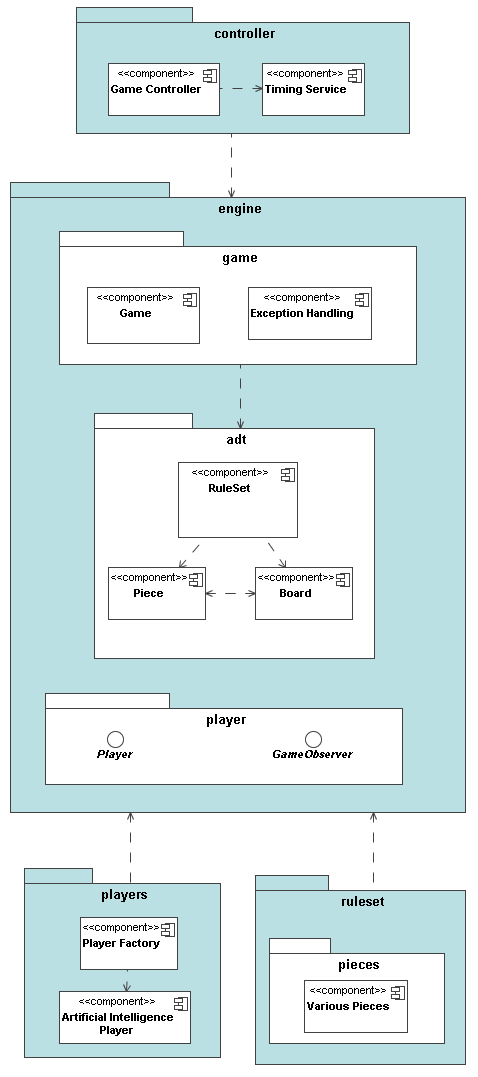
\includegraphics[width=220pt]{img/component-diagram.png}
						\caption{\emph{Pawned}'s Implementation Diagram}
	  			\label{implementation-diagram}
		   \end{center}
	\end{figure}
	
	\begin{description}
		\item[Controller Layer] The controller layer provides the asynchronous messaging turn request
														and notification system. The abstract
														\emph{Controller} defined in Section \ref{problem-analysis} is contained 
														within this layer, along with the timers and asynchronous messaging utilities
														required to query and inform users of incoming events. %%XML factories
		\item[Game Layer] The game layer provides the mechanism for board-player interaction under the
											rules and regulations of the rule set. The abstract \emph{Game Model} defined
											in Section \ref{problem-analysis} is contained within this layer
		\item[Programmatic Interface] This layer contains the interfaces and abstract classes that need to be subclassed 
											in order to implement a new game. They describe the basic rules, boards, and pieces
											that are allowed in the game, and provide a contract with the \emph{Game Execution 
											Environment} that permit the operation of the top layers, along with the specification 
											of the contracts that objects have to fulfill in order to participate in games, via the 
											\textbf{Player} and \textbf{GameObserver} interface.											
		\item[Developer Utilities] A set of prefabricated pieces, boards, and players that conform with the 
															 specification of the published \emph{API} and that can be used 
															 in the development of games. 
	\end{description}	
	
	
	These layers, along with their general modular dependencies, are presented as an implementation 		
	diagram, in Figure \ref{implementation-diagram}, along with the modular structure of the
	application.
	 	\subsection{Programmatic Interface}
	 		\paragraph{Contents}
		 		The programmatic interface layer is found in the \texttt{engine.adt} package. 
		 		It defines the contract between the game developer and the execution environment.
		 		Its components classes are \texttt{Action}, \texttt{Board}, \texttt{Parser}, 
		 		 \texttt{Player}, \texttt{Ply}, \texttt{Piece}, and \texttt{RuleSet}.  See Section 
		 		 \ref{player-observer} for a discussion of \texttt{Player} and \texttt{GameObserver}

		\begin{figure}
			\begin{center}
				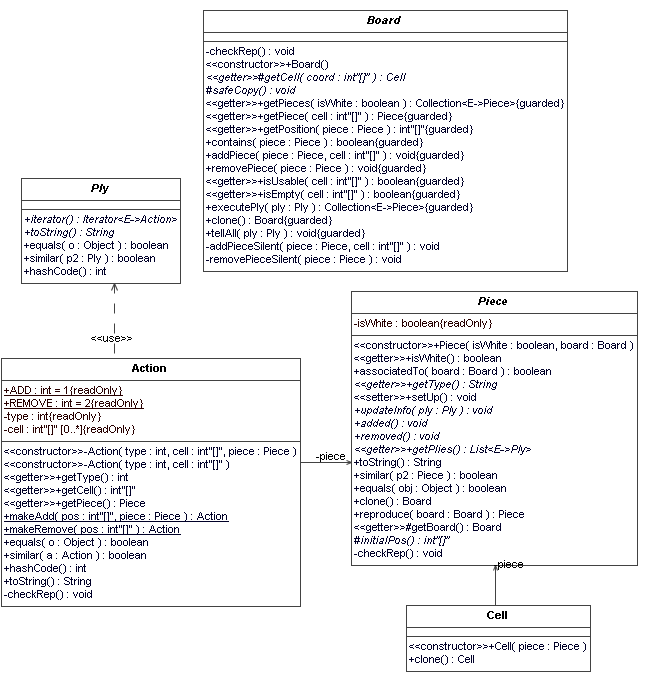
\includegraphics[width=270pt]{img/board-piece-action-ply.png}
						\caption{Board-Piece-Action-Ply interaction}
	  			\label{board-piece}
		   \end{center}
	\end{figure}
		 		 
	 		 \subsubsection{Board-Piece interaction for sequential games}\label{board-discussion}
	 		 		There exist several different ways to implement a piece manipulation scheme within a board. 
	 		 		For example, an implementation for \texttt{Board} could contain methods such as 
	 		 		\texttt{makeMove(int[] from, int[] to)}, \texttt{castle()}, etc.
	 		 		The board would then be in charge of determining whether the moves are legit, and
	 		 		executing them. However, this would mean that the board would be forced to be 
	 		 		eternally coupled with a particular rule set, and it would be unpractical for any 
	 		 		game-neutral agent to translate generic moves into game-specific method calls to a particular
	 		 		board. For that reason, such an implementation would greatly harm extensibility. 
	 		 		
	 		 		Another possibility could be for each piece to contain the board they are currently in, 
	 		 		and then to ask each piece for the information that is relevant to them. For example, 
	 		 		a king in \emph{6.170 Antichess with Encastling} would query a rook for information 
	 		 		on whether he has moved. Then, based on this information, the king would determine whether
	 		 		he can or cannot castle. However, since a board that holds different types of pieces can 
	 		 		only hold a general object of type \texttt{Piece}, and not particular subclasses, 
	 		 		each object of type \texttt{Piece} would require, in this example, to contain an implementation for
	 		 		\texttt{boolean hasMoved()}. Once more, this solution is impractical for a generic game environment, 
	 		 		where each piece could require arbitrary types of information about the other pieces and their 
	 		 		movements.   
	 		 		
	 		 		Yet another alternative would consist of having only a global ruleset, in charge of computing 
	 		 		all the possible moves given a board configuration. This option brings the advantage that
	 		 		only one instance of each piece type would be required, since pieces would not be required
	 		 		to hold any game-specific state. However, the desired states for any given type of piece
	 		 		would still be held inside the rule set. Then, all the information regarding each piece 
					would be stored in a single location, making it difficult to maintain and extend. During development,
					a benchmarking scheme was devised, in which several pieces with certain information were instantiated.
					Afterwards, the performance in time and memory was compared with the creation of a single object
					storing all the information. The result threw no significant difference between both methods.
					
					For these reasons, \emph{Pawned} requires the pieces to be aware of the state of the board, 
					and then compute their valid moves, in the way introduced by Section \ref{problem-analysis}.
					The design and implementation details for these scheme are presented in the following sections.   
					 
	 		 \subsubsection{Board}
	 		 		\paragraph{Description}An object of type \texttt{Board} represents an N-dimensional game board.
	 		 													 That is, a set of cells arranged in some order. A 
	 		 													 \texttt{Cell} is a simple data type that 
	 		 													 in a board may contain at most one \texttt{Piece}. 
	 		 													 To refer to a cell within the board, its position 
	 		 													 must be specified. A cell's position is determined by $n$ 
	 		 													 integers, which specify the coordinates of the cell 
	 		 													 in an $n$-dimensional board. 
	 		 													 
	 		 													 It should be noted that not all possible combination of $n$
	 		 													 integers are necessarily associated to a cell. If a sequence
	 		 													 of $n$ integers $(k_1, k_2, \cdots, k_n)$ is unusable. 
	 		 													 
	 		 													 A board contains a set of pieces, 
	 		 													 each inside of some distinct cell. A usable cell might thus 
	 		 													 be empty or occupied by a piece. If a cell is usable and empty, 
	 		 													 then a piece can be added to this cell. 
	 		 													 
	 		 													 A board can execute valid \texttt{Ply}, a sequence
	 		 													 of additions and removals of pieces within a board. (See Section 
	 		 													 \ref{PlyAction}). A ply is valid with respect to a 
	 		 													 \texttt{Board} if the set of actions it defines can possibly 
	 		 													 be executed given the current board configuration.   

					\paragraph{Class type choice} \texttt{Board} is an almost fully implemented abstract class. 
																				Most of the operations can be implemented in terms of the 
																				\texttt{Cell getCell(int[] coord)}. A distinct board can be built
																				by implementing the previously mentioned method. In this way, 
																				an appropriate cell fetching mechanism can be used to retrieve
																				a particular cell. For example, in the case of a chess rectangular
																				board, the representation for a board could consist of an eight 
																				by eight array of cells, whereas a very large board could use 
																				other mechanisms for storage, such as a hash table. With this
																				design choice, boards can also have any arbitrary shape, 
																				dependent on the implementatino of the particular 
																				\texttt{Cell getCell(int[] coord)} method. 
																				
																				A mapping from pieces to its coordinate is kept in the abstract
																				class in order to implement the \texttt{int[] getPosition(Piece piece)}
																				method efficiently. This optimization is very useful, since 
																				a game ruleset and the pieces themselves are expected to query the
																				board often for this information. 


					\paragraph{Important features and design choices}
												A \texttt{Board} is synchronized. This allows the board to be accessed in an
												asynchronous fashion. For \emph{Pawned}, this is a necessary condition, since
												players and observers could potentially request and read information from the 
												board while the controller is executing moves on it. Additionally, the set
												of pieces of a color that can be retrieved by the board's 
												\texttt{Set<Piece> getPieces(boolean colorIsWhite)} will not change even a ply 
												is executed, in order to ensure that a caller can safely iterate over it. 
																								
												A \texttt{Board} is clonable, in a deep copy sense. A deep copy is required in order
												to ensure that board manipulations in a copied board are independent of the initial 
												board, so the boards cannot share a reference to a same object, since in doing so, 
												any modification in one board would have side effects on the other. The implementation of this 
												functionality is non trivial at the abstract class level, 
												since in order to deep copy, a board would require information 
												about its representation, which is not readily available in this case. 
												
												A possible solution for this situation could be to utilize \emph{Java Reflection} to dynamically
												obtain the fields from the subclasses, and set the copy's fields to be clones of the initial fields.
												However, this would require all of the components of the extending classes to be clonable, and would
												also require a very stringent contract between this class and its implementing classes. Therefore, 
												in order to solve this issue, each board that extends \texttt{Board} must clone its representation 
												on request. Since each implementation should know how to deep copy itself, the clone method
												of the generic board can rely on these side effects to successfully deep copy the board. 
												After it has done so, the board can be safely cloned. Since the latter method is less error prone and
												requires less processing, this is the method chosen for \emph{Pawned}. Although the method is
												protected, therefore exposing it to potential external unwanted calls, the effects on a board
												would not disrupt its normal functioning, since the representation held after the method call would 
												represent the exact same state as before. Therefore, there is no danger in exposing this method. 
												
												The board implements a notification mechanism for its subscribed pieces. This notification mechanism
												informs the pieces whenever they are added or removed from the board, and also whenever a ply is 
												executed in the board the pieces currently populate. With the use of the \emph{Observer} pattern 
												in this case, pieces can gracefully receive notifications that they can use in order to process
												their corresponding valid plies. For example, a king in \emph{6.170 Antichess with Encastling}
												would be able to monitor its rooks, keeping a record on whether it is allowed to castle or not. 
												With the ply notification system, the king can notice when the rook (or the king itself) has
												moved, and then update its state to no longer publish castling as an allowed move, in case
												all the other castling conditions apply. 
												
												In order to achieve this functionality, pieces must be associated with a single board. There
												are several reasons for this requirement. On one hand, a piece can only be playing a game
												in one place at a time. If no association were required, the piece could potentially be
												added to more than one board, getting notifications from both and not being able to determine
												which call came from what board, and thus disrupting its normal functionality. Additionally, pieces 
												are notified whenever they are added or removed, for situations where in-game addition of
												pieces is allowed.  	
												
												Boards make use of the exceptions provided in \texttt{engine.exception} to indicate 
												illegal calls or requests to the board. Since these errors could occur at several
												different points, and because of the need to distinguish them from other types of 
												runtime exceptions, \texttt{InitialPositionException}, \texttt{InvalidBoardException}, 
												and \texttt{UnusableCellException} provide more clarity and specificity when 
												each error is thrown. 											
																								
	 		 \subsubsection{Piece} 
	 		 		\paragraph{Description}A \texttt{Piece} represents an object that is placeable in a cell 
	 		 									within a specific \texttt{Board}. \texttt{Pieces} can be asked to
	 		 									return a list of the valid \texttt{Ply} that they can perform. It
	 		 									also contains information about its color, 
	 		 									along with its initial position in a 
	 		 									specific type of board according to the local rules of the game. 
	 		 						
	 		 		\paragraph{Class type choice}	Piece is an abstract class. This is because, depending on the 
	 		 									\texttt{RuleSet}, each piece needs to be aware of what moves 
	 		 									are valid given their position. However, some methods are common
	 		 									to all possible pieces, such as \texttt{boolean isWhite()}, 
	 		 									\texttt{void setUp()}, \texttt{void associateTo(Board board)},
	 		 									which specify common mechanisms for determining a piece's color,
	 		 									setting it up given a concrete subclass-provided initial position, 
	 		 									and an board association procedure. 
	 		
	 				\paragraph{Important features and design choices} 
	 											Once a piece is set up in a board, it automatically subscribes to 
	 											the board's messaging service, engaging in a doubly coupled 
	 											observer-broadcaster relation. This mechanism allows the pieces
	 											to receive information about the game, for the reasons specified
	 											in Section \ref{board-discussion}. 
	 							
	 											An initial consideration regarding pieces is the constant assumption 
	 											that only two types of piece exist, either black-colored pieces
	 											or white-colored pieces. By convention, ``white'' is the name
	 											of the principal player in a two-player sequential game, while
	 											``black'' is the name of the secondary player. For example, in chess, 
	 											the white player can be considered the principal player since it 
	 											moves first. A game such as a four-player chess would violate the
	 											assumption of dichromatic pieces. In order to solve this situation, 
	 											a player number (as opposed to \texttt{boolean isWhite}) would be 
	 											required on each of the player number descriptions. However,
	 											this decision would hurt readability of the code. In the case that
	 											such an extension were required, a simple code refactoring would 
	 											allow a transition from a 2 player sequential game to an n player
	 											sequential game.
	 						
	 											Since a piece has to be associated to a particular instance of a board, 
	 											it is unfeasible to clone a piece, since it would be impossible to set the
	 											cloned piece to be associated with a different board, so pieces would not
	 											be clonable and placeable on different boards. For that reason, 
	 											\texttt{Piece reproduce(Board board)} acts as a cloning mechanism, except 
	 											that it provides the functionality of changing the associated board to 
	 											the specified board, thus making piece ``cloning'' feasible. 
	 											
	 											Since several pieces in a board could be identical (e.g. two black pawns
	 											in a chess board), there is no way to distinguish them by just observing
	 											their characteristics and specfield representations. Therefore, the concept
	 											of referenciaql equality for comparison is required in order to ensure
	 											correct behavior of the board. However, a mechanism to compare whether
	 											two pieces are of the same type and the same color is provided under
	 											the name of \texttt{boolean similar(Piece)}. This method allows the comparison
	 											of two pieces, even when they are associated to distinct boards, and the comparison
	 											of plies that represent similar end results, but contain a referencially unequal 
	 											piece in them. See Section \ref{PlyAction} for further discussion on ply-action-board
	 											interactions. 
	 											
	 											In order for the piece to contain all of the information related to itself, 
	 											a piece holds information on the location it should set itself up when a game is
	 											started. Although the global rule set could contain this information, this 
	 											centralized storage of information would bring difficulties in maintaining code, 
	 											for different parts of the piece behavior would be maintained on different places.
	 											The piece therefore has information about the set of possible cells that it could 
	 											be placed on. Since these cells can be more than one, this information cannot only be
	 											stored in a field. The piece provides a \texttt{void setUp()} method on which
	 											the piece automatically detects where it can be placed, or throws an exception when
	 											it is incapable of doing so. With this information, all of the pieces of a game 
	 											can be setup by an agent that has no knowledge about the initial positions of the
	 											pieces. 
	
												A mechanism is needed to communicate the piece type to the game (for saving and piece
												generating purposes, for example). For this reason, each piece provides
												a unique identifier of itself via its type. Since it might still be possible that more
												information wants to be conveyed about the pieces in a string representation (e.g.
												``a black pawn located at e8'', the \texttt{String toString()} method is not 
												necessarily equal to a \texttt{String getType()} call, which can be useful 
												for development or message display purposes. 
												
												Finally, \texttt{List<Ply> getPlies()} is one of the central functions of the piece.
												Possessing all the necessary information from the board and its movements, via the
												inform mechanisms discussed above, a piece object can make a decision 
												regarding which plies could be executed on it. These returned plies are filtered only 
												regarding the local rules for the piece, and not with the general state of the game.
												For example, the restriction on  \emph{ 6.170 Antichess} that no piece can move when 
												a player is in chess unless such a move releases the king from check is not a local rule,
												so it is not enforced by the local \texttt{List<Ply> getPlies()} call. 
	 												 											
			\subsubsection{Ply and Action}\label{PlyAction}
				\paragraph{Description}	An \texttt{Action} represents an atomic change in a board. There are only 
																two types of actions: add, and remove. An add action adds a piece to a cell 
																in a board. A remove action removes the piece from a cell. An action therefore
																includes information about its type, the cell, and the piece (if any, it refers to)
																
																Any possible ply in a sequential game can be expressed as a sequence of actions. For 
																that reason, \texttt{Ply} is simply a sequence of actions that represent
																a player's turn in a sequential game.  
				\paragraph{Class type choice} 			
																Action is a concrete class, since \emph{Pawned} assumes that
																the atomic game movement units are add and remove from the board. 
																Although there are some other possibilities for atomic actions, such as 
																``destroy cell'', which renders the cell in question unusable, no direct support
																is provided for this type of action. However, its implementation would only require
																a modification of the specification and implementation of \texttt{Action} and 
																\texttt{Board}. 

	 			\paragraph{Important features and design choices} As discussed previously, \emph{Pawned} uses
	 								plies to express any type of board manipulation necessary, thereby ensuring extensibility.
	 								
	 								One of the issues that arise while implementing this data type is the concept of ply equality.
	 								A natural implementation of ply equality would be that a ply is equal to another whenever, if
	 								both plies were applied to a board with the same configuration, it would yield the same final 
	 								configuration. However, some complicated issues arise from this definition. Since the ply is
	 								applicable for any given board, the most naive implementation of the algorithm would require
	 								executing both plies to be compared on every possible board, applying both plies to board
	 								clones and then determining whether the new boards are equal.
	 								
	 								For example, consider the following two plies (assuming a 2D board for clarity in this document)
	 									\begin{description}
	 										\item[Ply 1]
	 											\begin{enumerate}
	 												\item Remove piece from $b5$. 
	 												\item Remove piece from $a1$.
	 												\item Add last piece removed. 
	 											\end{enumerate}
	 										\item[Ply 2]
	 											\begin{enumerate}
	 												\item Remove piece from $b5$.
	 												\item Remove piece from $a1$.
	 												\item Add last piece removed to $b5$. 
	 												\item Remove piece from $a1$. 
	 												\item Add piece $x$ to $a1$.
	 												\item Remove piece from $a1$. 
	 											\end{enumerate}
	 									\end{description}				
		In this case, these plies are not equal, since the final boards will be equal only if $a1$ is initially empty.
		Therefore, an algorithm would require to verify each action where the board at the relevant cell is both empty 
		and full, thus resulting in an exponetial explosion. Additionalyl, the pieces making use of a particular ply 
		would be required by the specification not to assume a particular way to represent an equal ply, thus forcing them 
		to provide code generic enough that could work for any possible expression of a given ply. In order to control this 
		problem, the pieces (as members of a rule set) can make assumptions about the predefined structure of the plies
		within that rule set. Then, by assuming the structure of the plies in the game, the code in the piece is greatly
		simplified. 
		
		In the same way as the pieces, a test for similarity (and not just strict equality) is provided. 
		
		Finally, the ply must provide a string representation of itself, in order to be reproducible by the factories 
		in the rule set. 
	
		\subsubsection{Parser}
			\paragraph{Description and Type} A parser is convertion from a string representation of a coordinate to 
											to and from the coordinate it represents. This mechanism is useful for saving and loading
											purposes, along with the \texttt{String getType()} and \texttt{String toString()} methods in 
											\texttt{Piece} and \texttt{Ply}, respectively.  
		
											The parser is an interface, since the conversions are fully game-dependent. 
											
		\subsubsection{RuleSet}
			\paragraph{Description} A \texttt{RuleSet} represents a set of local and global rules upon which a game can be
													fully operated. That is, a \texttt{RuleSet} is a mechanism for determining and creating all of 		
													possible plies, pieces and boards supported by a particular game, as well as to indicate the set of 
													possible plies and \texttt{GameTermination} that can happen given a board configuration. Since this
													method is fully dependent on each game, \texttt{RuleSet} is an interface. The decoupling between 
													the rules and the game execution comes mainly from the treatment of any given ruleset through 
													this interface. Since a \texttt{RuleSet} is defined almost exclusively in terms 
													of its relationship with game, it is fully discussed in Section \ref{game-layer}.   
			\paragraph{Important features and design choices} The \texttt{RuleSet} can be thought of as the 
													pluggable brain for the \emph{Game Execution Environment}. For that reason, 
													it must provide all the information the platform requires in order to correctly 
													carry out a game. 

													A \texttt{RuleSet} provides a set of factories, namely a \texttt{PieceFactory}, a 
													\texttt{BoardFactory}, and a \texttt{PlyFactory}. This factories are used by the
													
													For a discussion of the interactions between the game layer and this
													interface, please refer to Section \ref{game-discussion}. 
													
		\begin{figure}
			\begin{center}
				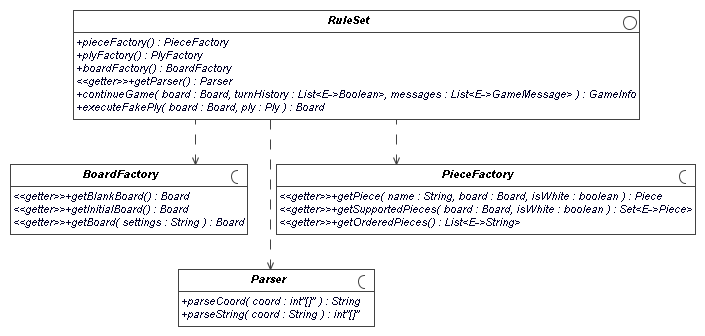
\includegraphics[width=300pt]{img/ruleset.png}
						\caption{RuleSet and its factories}
	  			\label{ruleset}
		   \end{center}
	\end{figure}
													
			
		\subsection{Game Layer}\label{game-layer}
	 		\paragraph{Contents}
		 		The game layer is found in the \texttt{engine.game} package. 
		 		It is the mechanism under which a board can be manipulated according to the rules
		 		specified by a ruleset. Further, it also allows the storage of the game state. 
		 		Its components classes are \texttt{Game}, \texttt{GameInfo}, \texttt{GameMessage}, 
		 		and \texttt{GameTermination}. 
	
		 		 \subsubsection{Game-RuleSet interaction for sequential games}\label{game-discussion}
					The \texttt{Game} is in charge to keep the state in the game. However, the ruleset can be
					called from a static context. Although \texttt{RuleSet} itself is an interface, so 
					it therefore must provide non-static methods, its behavior is not expected to change depending
					on its state. In general, a single ruleset can service several games of the same type happening 
					at the same time. For example, when an Artificial Intelligence player is pondering moves, 
					he does not need to create a ruleset for each of the possibilities explored, but rather
					call the same ruleset that the game is associated with. 

					By keeping a static communication with the \texttt{RuleSet}, resources can be optimized, by not
					requiring several instantiated objects to be present in order to use the game. However,
					this design choice is not strictly enforced. A rule set can be instantiated and can keep a game
					dependent state, if it considers necessary. In this way, rule sets can be optimized 
					in the case that they are very resource intensive. Regardless of this, \emph{Pawned}
					provides solutions for some amount of information storage, even with static methods, via 
					its \texttt{GameMessage} system.  
									
					The \texttt{RuleSet} and the \texttt{Game} synchronize information every time a move is executed. 
					The \texttt{RuleSet} receives a call to its 
					\texttt{continueGame(Board board, List<Boolean> turns, List<GameMessage> messages)} method.
					With this information, the \texttt{RuleSet} returns a \texttt{GameInfo} bean, which 
					contains information about the current state of the game. 

					\paragraph{GameInfo} is a bean that contains information about a \texttt{Game} at a particular
					state. This information includes the list of valid plies for the current board configuration, the
					player who should execute the next move, and a list of game messages that are associated with the new 
					state. However, a \texttt{GameInfo} object cannot represent a terminated state. Therefore, 
					\texttt{GameTermination} objects are the representatives of the state. 					

					\paragraph{GameTermination} This is a \texttt{Throwable} object used to indicate that a \texttt{Game}
					has terminated, due to a termination condition. It contains information about who won the <tt>Game</tt>
					(or if it was drawn), and why.
					
					Whenever a game has finalized, a \texttt{GameTermination} is thrown instead of returning 
					a \texttt{GameInfo} object. This structure allows game terminations to be easily detected and 
					propagated automatically along several method invocations, if necessary; it also allows 
					the separation of termination and active states, for a cleaner implementation. 
					  
					 \paragraph{GameMessage} objects describe additional information about a current game state. 
					 This information can be used to either notify users of relevant states in which they are
					 involved, or for use in the ruleset for optimization purposes. For example, in a \emph{Connect 4}
					 game, the ruleset might be interested in knowing the previous plies that were executable, 
					 in order to check those pieces for path formations, as opposed to the complete board. In the same 
					 way, a game of \emph{Chess} implementing draw conditions could make use of this messaging 
					 service to persist some string representation of previous board states, in order to validate whether
					 a given board configuration has been repeated or not. 
					  
		\begin{figure}
			\begin{center}
				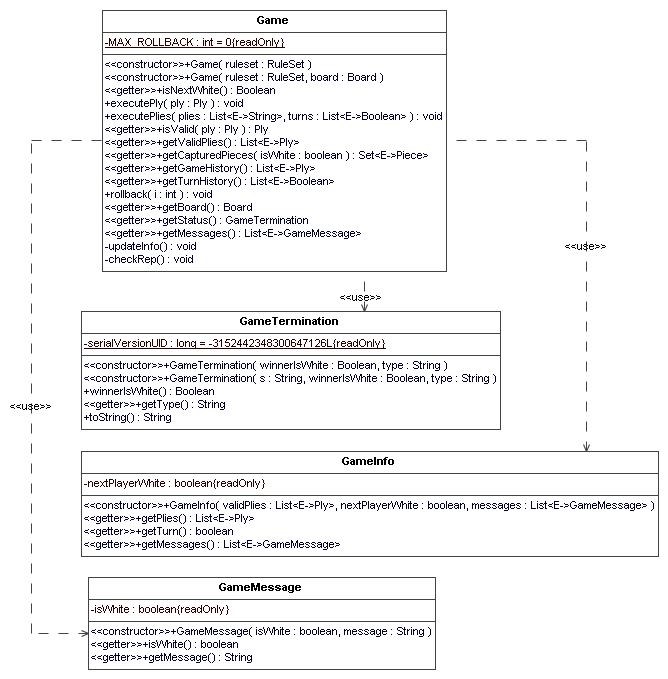
\includegraphics[width=250pt]{img/game.png}
						\caption{Game and its supporting classes}
	  			\label{ruleset}
		   \end{center}
	\end{figure}
					   
				\subsubsection{Game}
					\paragraph{Description} As specified previously, \texttt{Game} provides the central mechanism for 
						game control. It contains information about the game rules using a rule set. Additionally,
						it maintains a board representing the current board configuration, and a set of collected pieces.
						A piece $p$ is collected if, after a ply has been executed, whenever $p$ was contained in the board
						before the ply was executed and $p$ is not contained in the board when the ply was executed, 
						$p$ is a collected piece by the ply. The state for a game can be either active or terminated. Game
						is a concrete class. 
						
			\paragraph{Important features and design choices} The \texttt{Game} can be thought of as a proxy 
						between a synchronous ply executor and a board, ensuring that the board is manipulated according
						to the rules, and keeping the relevant information about the game history and status. 
						
						Since a \texttt{Game} possesses no prior knowledge of the game being played, it must depend 
						entirely on the rule set for game specific decisions. All of the executed plies result in a call 
						to the ruleset, from which the game updates its state. All of the methods provided by this class are 
						obtained in this fashion. However, \texttt{void executePlies(List<Ply> plies)} builds a game without
						consulting with the ruleset. This method can be used when a set of plies that are known to be valid 
						need to be executed without the overhead produced by the constant calls to the ruleset. The 
						pieces, due to the board's notification mechanism, would still be able to hold all the information 
						they require for their proper functionality. 
						
						In order to guarantee that a game runs adequately, it would be necessary to query the ruleset after
						every move is made. This condition does not impose much additional overhead for a chess game
						of regular length. However, since the average length for all types of game is not known, 
						and neither is the amount of processing required after each move for each particular ruleset, 
						it is impossible to predict how much overhead would result in general. An extension on this program could
						provide a boolean as a parameter for this method, so that the caller can decide whether he desires
						to guarantee that all the plies are valid. 
						
						All the collections returned by this class are unmodifiable, in order to prevent modifications. See 
						\ref{final-extensibility} for a discussion of the protection against undesired mutations 
						in \emph{Pawned}. 
											
										
		\subsection{Controller Layer}
			\subsubsection{Contents}
				The controller layer contains the classes \texttt{Controller},\texttt{Stopwatch}, and \texttt{XmlFactory}. 

			\subsubsection{Player and GameObserver - Controller Relation}\label{player-observer}
					\paragraph{Description} The controller provides asynchronous communication between the players and 
								the game. In other words, the \texttt{Controller} is in charge of providing a guarantee
								of synchronized calling to game, as well as handles the ply retrieval and information to and 
								from the players. In order for the \texttt{Controller} to achieve this goal, two interfaces: 
								\texttt{Player} and \texttt{GameObserver} are defined. 
								
								A \texttt{GameObserver} is an entity that can be subscribed to 
 								the listening message queues in a controller. An observer receives notification regarding 
 								the plies that are executed on a given gamem, along with information regarding the termination of the game.
 								
 								A \texttt{Player} is a type of game observer that, apart from being informed about the game status, 
 								it gets queried for moves to be executed within the game. 
 								
					\paragraph{Design Decisions} 
																The use of the observer pattern allows an easy solution to the problem of notifying 
																observers of modifications in the shared game. There are various other alternatives
																that were considered before the constructions of these interfaces.
																
																For example, the controller could work in a synchronized fashion, providing methods
																that allow another agent to determine when to make moves and when to obtain moves from 
																computer players. In this case, an interface (such as the GUI) would be in charge of 
																managing the workflow in the application. An immediate advantage to this
																approach is the reduced number of threads that are required. However, this approach 
																must limit the application to a simple desktop human-computer game. This is because
																the user interface would be empowered to input its own moves, and to ask the
																controller for the AI Player's moves, implicitly assuming that the only possible
																players are these. 
																
																Under \emph{Pawned's} archiecture, a variety of player types and interfaces can 
																be easily implemented. For example, any class implementing \texttt{GameObserver}
																can participate as a game listener. A large amount of services can then be added to games
																in this fashion, such as logging services, game analyzers, artificial learners, etc.
																 
																Similarly, different types of players can easily be added to the architecture without 
																any modification. For example, the notion of an Internet Player, a player that connects
																to the controller via Internet in order to play a game, or a plugin for connection with 
																existing chess servers are all easy to implement under the structure provided by 
																\emph{Pawned}.

			\subsubsection{Controller}
				\paragraph{Description} A controller is a the communication link between the players and a game. 
																It is also responsible for saving the game using the information contained
																in the Game, as well as managing the time in the game. 
				\paragraph{Threading issues} A controller consists of at most four distinct threads. Two of these
												threads are devoted to keeping the time remaining for each of the players, and 
												ending the game as soon as the time expires. A third thread constantly executes the
												\texttt{TurnCycle}, the ply dispatcher in charge of retrieving and executing plies for the 
												players, as well as informing each of the observers of an executed move. 
												
												There are, once more, several implementation possibilities for the controller regarding its
												interaction with the players, assuming an asynchronous communication. For example, each call to 
												an \texttt{inform(String ply)} could come from a pool of threads. This mechanism would be efficient, 
												especially in the case where several observers are expected. Under these conditions, a loop that waits
												for each of the observer's \texttt{inform(String ply)} method to terminate could lead to very long wait 
												times, or even to an unrecoverable state. However, there is a tradeoff with using this approach. 
												By separating the calls to \texttt{inform(String ply)} from the \texttt{submitPly()} dispatcher -- 
												that is, from the mechanism in charge for retrieving the moves from the players --, then it is no 
												longer possible to guarantee that a player whose turn it is to play will get notified of all the plies 
												that were previously executed before it is his turn to move. 
												
												Since the lack of this guarantee would require more complicated information handling, the inform
												mechanism is carried out in a single thread. However, a change to another type of implementation 
												would be very easy to obtain. 
												 
				\paragraph{XML Saving and Loading} 
					In order to save an XML file, the controller requires to provide information about the piece configuration, 
					the move history, the turn history, and the time at which each ply was executed. This information is all contained
					in the game. Since each of the plies and the pieces in the board have a particular string representation, this
					is used to persist them into the XML file. Further, the ruleset provided parser is used to parse the cell coordinates
					into the game-specific representation of the cells. Additionally, whenever a game is terminated, this information 
					is also readily available as a \texttt{GameTermination}.Finally, the ruleset provides its own 
					String representation, completing the requirements for the information to be saved in the XML file. In this way, the 
					XML file can be generated with no ambiguity. 
					
					In order to load a game from XML file, it is necessary to create a new controller using a constructor that takes an 
					XML file as a parameter. Once the controller has knowledge about the ruleset to be used, each of the pieces
					can be generated from the ruleset's piece factory. Similarly, each of the ply 
					representations can be translated into actual plies using the ruleset-provided ply factory. 
		

			\subsubsection{StopWatch} 
				\paragraph{Description} A \texttt{StopWatch} represents a scheduling device that hsa
																the ability of being paused and resumed at any point during
																its execution. After its time expires, a \texttt{StopWatch}
																executes a \texttt{Runnable} task. 
				\paragraph{Important features and design choices} 
																The \texttt{StopWatch} class was designed in order to provide 
																the asynchronous notification to the players when the game has terminated
																due to time depletion. 
																
																An alternative to this implementation would be a non-threaded watch which
																verifies the remaining times only when moves have been executed. However,
																such a system would be confusing and would not allow for an immediate notification
																of loss by time depletion. 
																
																Further, the timer could be implemented at the User Interface level, only 
																notifying the controller about the time spent on each move. However, 
																since all the players would require to implement their own timing mechanism, this
																decision would lead to code repetition. Additionally, the responsibility delegated 
																to the players to provide the time consumption would require the strong assumption 
																that all of the players that could possibly be implemented will implement this 
																functionality correctly. These complications are removed when the controller itself handles 
																the time. There are, however, some considerations to be made when the communication time 
																between the controller and the player is expected to be long (e.g. using an Internet
																connection). These conditions could lead to a biased disadvantage against a player with a 
																slower connection. 
																
																
																It should be noted that the the \texttt{StopWatch} contains an inner \texttt{CheckRep}
																class. This is not only a static method as the regular checkReps, but rather a 
																representation invariant checker that keeps a state in order to determine whether
																the timewatch is preserving its state. 
																
																Since a \texttt{StopWatch} implementation relies on a constant update of 
																the amount of time remaining, we assert that, if $T_0$ is the 
																initial time at which the clock was started and $T_f$ is the actual time, 
																then let $\{r\}_n$ be the sequence of values set for remaining. Then 
																$ S = \sum_{k=2}^n ( r_k - r_{k-1} ) $ is the total time that has been
																consumed from the stopwatch.
																
																
																$$T_f = T_0 + S + P$$
																
																$P$ represents the total sum of the time when the stopwatch was paused. 
	
		\begin{figure}
			\begin{center}
				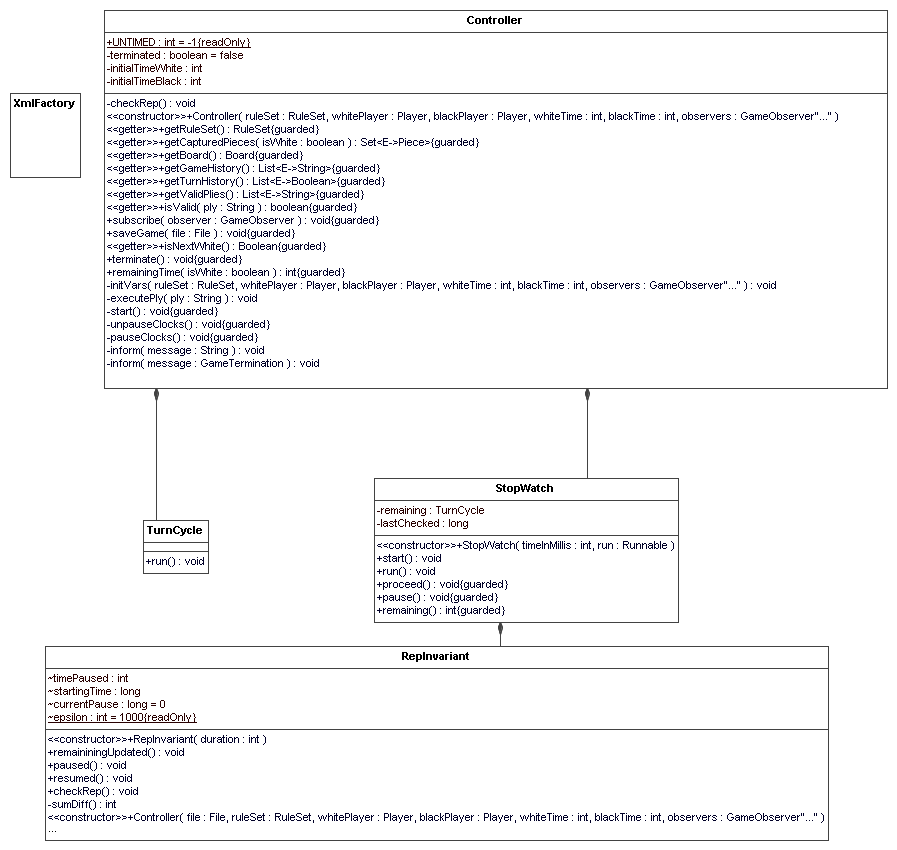
\includegraphics[width=270pt]{img/controller.png}
						\caption{Controller and its supporting classes}
	  			\label{controller}
		   \end{center}
	\end{figure}					

%\section{User interfaces}
%
\section{Standard Antichess}

Along with the \emph{Game Execution Environment}, \emph{Pawned} provides the implementations of a \emph{Standard 6.170 Antichess} and \emph{6.170 Antichess with EnCastle}. The pieces do not generally require the listener mechanisms inside
of board. This ruleset is provided under the \texttt{ruleset.antichess} packages. The set of pieces are contained in 
\texttt{ruleset.piece}, whereas the plies are contained in \texttt{ruleset.plies}. All of the previous are simple 
implementations of the required specifications detailed above. 


		\begin{figure}
			\begin{center}
				\includegraphics[width=300pt]{img/antichess.png}
						\caption{Antichess Ruleset}
	  			\label{controller}
		   \end{center}
	\end{figure}					
	

A generic antichess ruleset is extended by the encastling and the standard versions, each implementing \emph{Standard
6.170 Antichess} and {6.170 Antichess with Encastling, respectively}. This is because the only change resides in the
\texttt{PieceFactory}, which includes a different type of pawn and king, which have the faculty to castle and eat
en passant. 

